\documentclass[runningheads]{llncs}
\usepackage{graphicx}
\usepackage{float}
\usepackage[text={150mm,220mm},centering,nohead]{geometry}
\pagestyle{empty} 
\begin{document}
\title{\large{Service-Oriented Software Engineering (Project Proposal)}}
\author{}
\institute{}
\maketitle
\vspace{-1cm}
%-----------Please Do NOT change the content above.-----------------

%---------------------------------------------------------------------------------------------------------------------------------

%-----------Please write the project information here.---------------

\begin{center}
\Large{\textbf{Nice Title}} \\ % Please write your project tile in here
\vspace{0.2cm}
\large{\emph{Group Members (5): ZijiaHe, ChangXu, HongyiHuang, WangzhihuiMei}} \\%Please write names of your group members as well as the group number in here
\vspace{0.3cm}  
\end{center}

%-----------Please write the content of your research proposal from here.---------------
\noindent
\section{Data preparation}
There are 8 features (explanatory variables) and 1 label (response variable). These data are collected from actual patients and represent a task, usually performed by a human doctor, with the purpose of identifying the patients most likely to have diabetes in order to propose preventive measures.Some data values are 0, which is impossible, because these physical quantities cannot be 0 (for living people). Therefore, this has told us that we need to estimate these five columns. The scope of other variables seems to be reasonable.Next, we can calculate the relevant values to see the relationship between the characteristics and the results. Of course, correlation does not mean causality, but because we are building a linear model, correlation features may be useful for learning the mapping between patient information and whether they have diabetes.In problems with a large number of features, we can use relevant thresholds to delete variables. In this case, we may want to keep all variables and let the model decide which ones are related.In this brief exploratory data analysis, we learned about the two main aspects of data sets that can be used for modeling. First, we need to enter missing values in several columns, because these values are physically impossible. We can use the median method as a simple and effective way to fill the value of 0. We also learned that there is a correlation between features and responses, although the correlation is not strong. In addition, all features are at least slightly positively correlated with the result (whether or not the patient has diabetes).Next, in order to facilitate testing and training, we randomly select 75\% of the data set for training and 25\% of the data set for testing.
\begin{figure}[H]
\centering
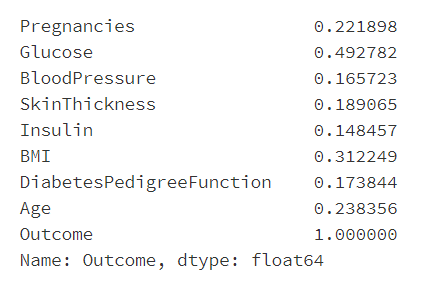
\includegraphics[width=3in]{1-2.png}
\caption{Correlation}
\end{figure}
\begin{figure}[H]
\centering
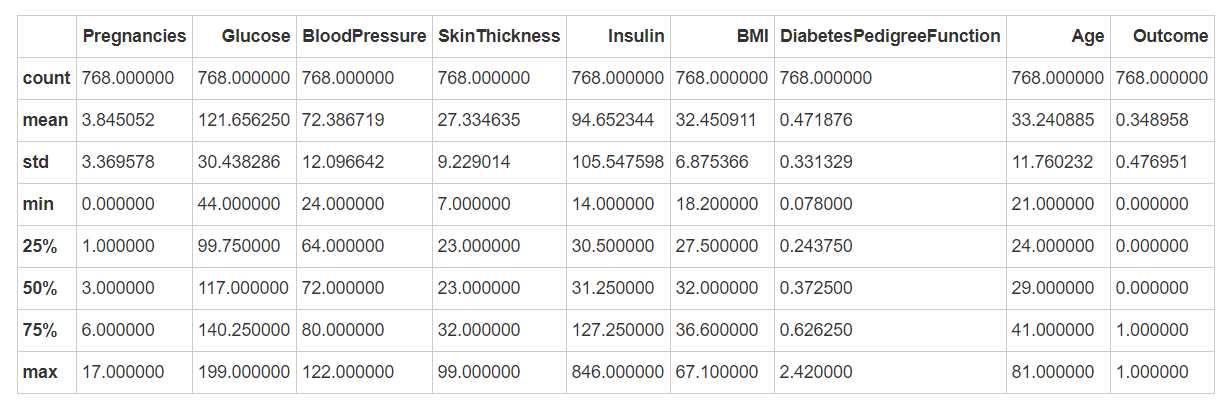
\includegraphics[width=6in]{1-1.png}
\caption{Data filled with missing values}
\end{figure}
\clearpage

\section{Classifiers}




%-----------Please write the content of your appendix (diagrams, figures, tables, etc) from here.---------------
\noindent 
\end{document}

